% SEC 1.1
\section{Systems of Linear Equations}
\name


\begin{exercise} % 1.1.1
	Solve the system by using elementary row operations on the augmented matrix. Follow the systematic elimination procedure described in this section.
	\[
	\systeme{
		x_1	+ 5x_2 =  7,
		-2x_1	- 7x_2 = -5}
	\]
\end{exercise}
\vfill


\begin{exercise} % 1.1.7 & 9
	The augmented matrix of a linear system has been reduced by row operations to the form shown. Continue the appropriate row operations and describe the solution set of the original system.
	\begin{multicols}{2}
		\begin{enumerate}[(a)]
			\item 
			$\begin{bmatrix}
			1 & 7 &  3 & -4 \\
			0 & 1 & -1 &  3 \\
			0 & 0 &  0 &  1 \\
			0 & 0 &  1 & -2
			\end{bmatrix}$
			\item
			$\begin{bmatrix}
			1 & -1 &  0 &  0 & -4 \\
			0 &  1 & -3 &  0 & -7 \\
			0 &  0 &  1 & -3 & -1 \\
			0 &  0 &  0 &  2 &  4
			\end{bmatrix}$
		\end{enumerate}
	\end{multicols}
\end{exercise}
\vfill


\newpage


\begin{exercise} % 1.1.13
	Solve the system. \\
	
	\systeme{
		x_1				-	3x_3 =  8,
		2x_1	+	2x_2	+	9x_3 =  7,
					 x_2	+	5x_3 = -2}
\end{exercise}
\vfill


\begin{exercise} % 1.1.19 & 21
	In each problem below, determine the value(s) of $h$ such that the matrix is the augmented matrix of a consistent linear system.
	\begin{multicols}{2}
		\begin{enumerate}[(a)]
			\item
			$\begin{bmatrix}
			1 & h & 4 \\
			3 & 6 & 8
			\end{bmatrix}$
			\item
			$\begin{bmatrix}
			1 & 3 & -2 \\
			-4 & h &  8
			\end{bmatrix}$
		\end{enumerate}
	\end{multicols}
\end{exercise}
\vfill


\hrule

\begin{exercise}[Extra Time] % 1.1.25
	Find an equation involving $g$, $h$, and $k$ that makes this augmented matrix correspond to a consistent system: \\
	
	$\begin{bmatrix}
	 1 & -4 &  7 & g \\
	 0 &  3 & -5 & h \\
	-2 &  5 & -9 & k
	\end{bmatrix}$
\end{exercise}


\newpage


% SEC 1.2

\section{Row Reduction and Echelon Forms}
\name[2in]

\begin{exercise} % 1.2.3
Row reduce the matrix to reduced echelon form. Identify (circle) the pivot positions in the final matrix and in the original matrix.
\[\begin{bmatrix}
	1 & 2 & 3 & 4 \\ 
	3 & 4 & 5 & 6 \\ 
	6 & 7 & 8 & 9
\end{bmatrix}
%\qquad\longleftarrow\qquad
%\parbox[]{3in}{Circle the pivot positions in the original matrix.}
\]
\end{exercise}
\vfill


\begin{exercise} % 1.2.9
Find the general solution of the system whose augmented matrix is given below. \\

$\begin{bmatrix}
0 &  1 & -6 &  6 \\
1 & -2 &  9 & -8
\end{bmatrix}$
\end{exercise}
\vfill


\newpage


\begin{boxthm}
\textbf{Theorem 2.}
\textbf{Existence and Uniqueness Theorem} \\
A linear system is consistent if, and only if, the rightmost column of the augmented matrix is \textit{not} a pivot column---that is, if, and only if, an echelon form of the augmented matrix has \textit{no} row of the form
$$ \begin{bmatrix}0 & \cdots & 0 & b\end{bmatrix} \qquad \text{with $b$ nonzero}.$$
If a linear system is consistent, then the solution set contains either 
\begin{enumerate*}[(i)]
	\item a unique solution, when there are no free variables, or
	\item infinitely many solutions, when there is at least one free variable.
\end{enumerate*}
\end{boxthm}


\begin{exercise} % 1.2.15
Suppose each matrix below represents the augmented matrix for a system of linear equations. Determine if the systems are consistent. If the system is consistent, determine if the solution is unique. (Leading entries marked with a $\blacksquare$ may have any nonzero value, and entries marked with a * may have any value including zero.)
\begin{multicols}{2}
	\begin{enumerate}[(a)]
		\item
				$\begin{bmatrix}
				\blacksquare	& *				& *				& * \\ 
				0				& \blacksquare	& *				& * \\ 
				0				& 0				& \blacksquare	& *
				\end{bmatrix}$
		\item	
				$\begin{bmatrix}
				\blacksquare	& *				& *	& * & * \\ 
				0				& \blacksquare	& *	& * & * \\ 
				0				& 0				& 0	& 0 & \blacksquare
				\end{bmatrix}$
	\end{enumerate}
\end{multicols}
\end{exercise}
\vfill


\begin{exercise} % 1.2.19
In the system of linear equations below, $h$ and $k$ represent real numbers.
\[\systeme[x_1,x_2]{
	 x_1	+	hx_2	= 2,
	3x_1	+	6x_2	= k
	}
\]
For each part below, choose values for $h$ and $k$ so that the desired property holds.
\begin{multicols}{2}
	\begin{enumerate}[(a)]
		\item The system has no solution.
		\item The system has 1 solution.
	\end{enumerate}
\end{multicols}
\end{exercise}
\vfill


\newpage


% SEC 1.3
\section{Vector Equations}
\name

\begin{boxme}
Usually vectors are depicted in bold font when in print (e.g. $\textbf{u}$, $\textbf{v}$, or $\vect{a}_1$). When writing by hand, you may wish to use the ``arrow'' notation for a vector instead (e.g. $\vec{u}$, $\vec{v}$, or $\vec{a}_1$).
\end{boxme}


\begin{exercise} % 1.3.3
	The vectors $\vect{u}$ and $\vect{v}$ are given, and $\vect{u}$ is displayed in the graph below.
	$$ \vect{u} = \begin{bmatrix} -1 \\ 2 \end{bmatrix}, \qquad
	\vect{v} = \begin{bmatrix} 2 \\ 3 \end{bmatrix}.$$
	\begin{multicols}{2}
	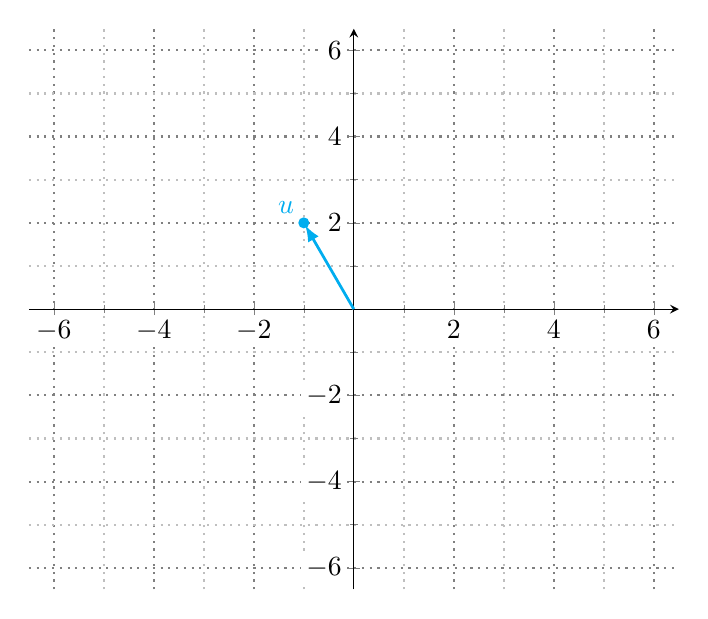
\begin{tikzpicture}
	% Set u and v
	\pgfmathtruncatemacro{\ux}{-1}
	\pgfmathtruncatemacro{\uy}{2}
	% Begin Axis
	\begin{axis}[axis x line=center, axis y line=middle,
	xmin=-6.5, xmax=6.5,
	ymin=-6.5, ymax=6.5,
	xtick={-6,-4,...,6}, ytick={-6,-4,...,6},
	ticklabel style={draw=none, inner sep=2pt, fill=white, text opacity=1},
	scale only axis, width=3.25in,
	grid=both, minor tick num=1,
	major grid style={line width=.8pt, draw=gray, dotted},
	minor grid style={line width=.8pt, draw=gray!50, dotted}]
	% Draw vector
	\draw[-latex, shorten >=.25ex, line width=1pt, cyan] (0,0) -- (\ux,\uy);
	\fill[cyan] (\ux,\uy) circle (2pt) node[above left, fill=white, rounded corners=0.2cm] {$\vect{u}$};
	\end{axis}
	\end{tikzpicture}
	
	\columnbreak
	
	The vector $\vect{u}$ is indicated on the graph to the left. Indicate the following vectors in a similar manner.
	\begin{multicols}{3}
		\begin{enumerate}[(a)]
			\item $\vect{v}$
			\item $-2\vect{u}$
			\item $\vect{u}+\vect{v}$
			\item $\vect{u}-\vect{v}$
			\item $\vect{u}-2\vect{v}$ 
		\end{enumerate}
	\end{multicols}
	\end{multicols}
\end{exercise}


\begin{exercise} % 1.3.5&9
	An augmented matrix for a system is given. For this problem, use the variables $x_1$ and $x_2$.
	$$\begin{bmatrix}
	-2 & 0 & -3 \\ 7 & -7 & 6 \\ 3 & 6 & 5
	\end{bmatrix}$$
	\begin{multicols}{2}
		\begin{enumerate}[(a)]
			\item Rewrite the augmented matrix as a system of linear equations. Do not solve the system.
			\item Rewrite the augmented matrix as a vector equation (using each column as a vector). Do not solve the system.
		\end{enumerate}
	\end{multicols}
	\vfill
	Note that in the first instance, the \textbf{rows} of the matrix are the important objects. In the second instance, we instead view the matrix as a linear combination of the \textbf{columns}.
\end{exercise}


\newpage


\begin{exercise} % 1.3.11
	Determine if $\vect{b}$ is in $\Span\{\vect{a}_1, \vect{a}_2, \vect{a}_3\}$. In other words, determine if $\vect{b}$ can be written as a linear combination of $\vect{a}_1$, $\vect{a}_2$, and $\vect{a}_3$.
	$$ \vect{a}_1 = \begin{bmatrix} 1 \\ -3 \\ 0 \end{bmatrix}, 
	\vect{a}_2 = \begin{bmatrix} 0 \\ 1 \\ 2 \end{bmatrix}, 
	\vect{a}_3 = \begin{bmatrix} 4 \\ -5 \\ 14 \end{bmatrix},
	\vect{b} = \begin{bmatrix} 4 \\ -1 \\ 22 \end{bmatrix}$$
\end{exercise}
\vfill


\begin{exercise} % 1.3.Custom
	For any nonzero vector $\vect{u}$ in $\R^2$, $\Span\{\vect{u}\}$ is a line passing through $\vect{u}$ and the origin, $\vect{0}$. See the picture.
	\begin{multicols}{2}
		\begin{center}
		\begin{tikzpicture}
		% Set u
		\pgfmathsetmacro{\ux}{4}
		\pgfmathsetmacro{\uy}{1}
		% Begin Axis
		\begin{axis}[axis x line=center, axis y line=middle,
		xmin=-6.5, xmax=6.5,
		ymin=-3.5, ymax=3.5,
		%		xtick={-6,...,6}, ytick={-3,...,3},
		ticklabel style={draw=none, inner sep=2pt, fill=white, text opacity=1},
		scale only axis, axis equal, height=2in,
		grid=major, grid style={line width=.8pt, draw=gray, dotted}]
		% Plot line
		\addplot[-,dashed, magenta, line width=1pt, domain=-6.5:6.5] {(\uy/\ux)*x};
		% Draw vector
		\draw[-latex, shorten >=.25ex, line width=1pt, cyan] (0,0) -- (\ux,\uy);
		\fill[cyan] (\ux,\uy) circle (2pt) node[above left, fill=white, rounded corners=0.2cm] {$\vect{u}=\begin{bmatrix} \ux \\ \uy \end{bmatrix}$};
		\end{axis}
		\end{tikzpicture}
		\end{center}
		
		\columnbreak
		
		If $\vect{u}$ and $\vect{v}$ are distinct nonzero vectors in $\R^3$, then $\Span\{\vect{u},\vect{v}\}$ \emph{may} be a plane passing through $\vect{u}$, $\vect{v}$, and $\vect{0}$ (as below)... but this is not always the case!
		\begin{center}
		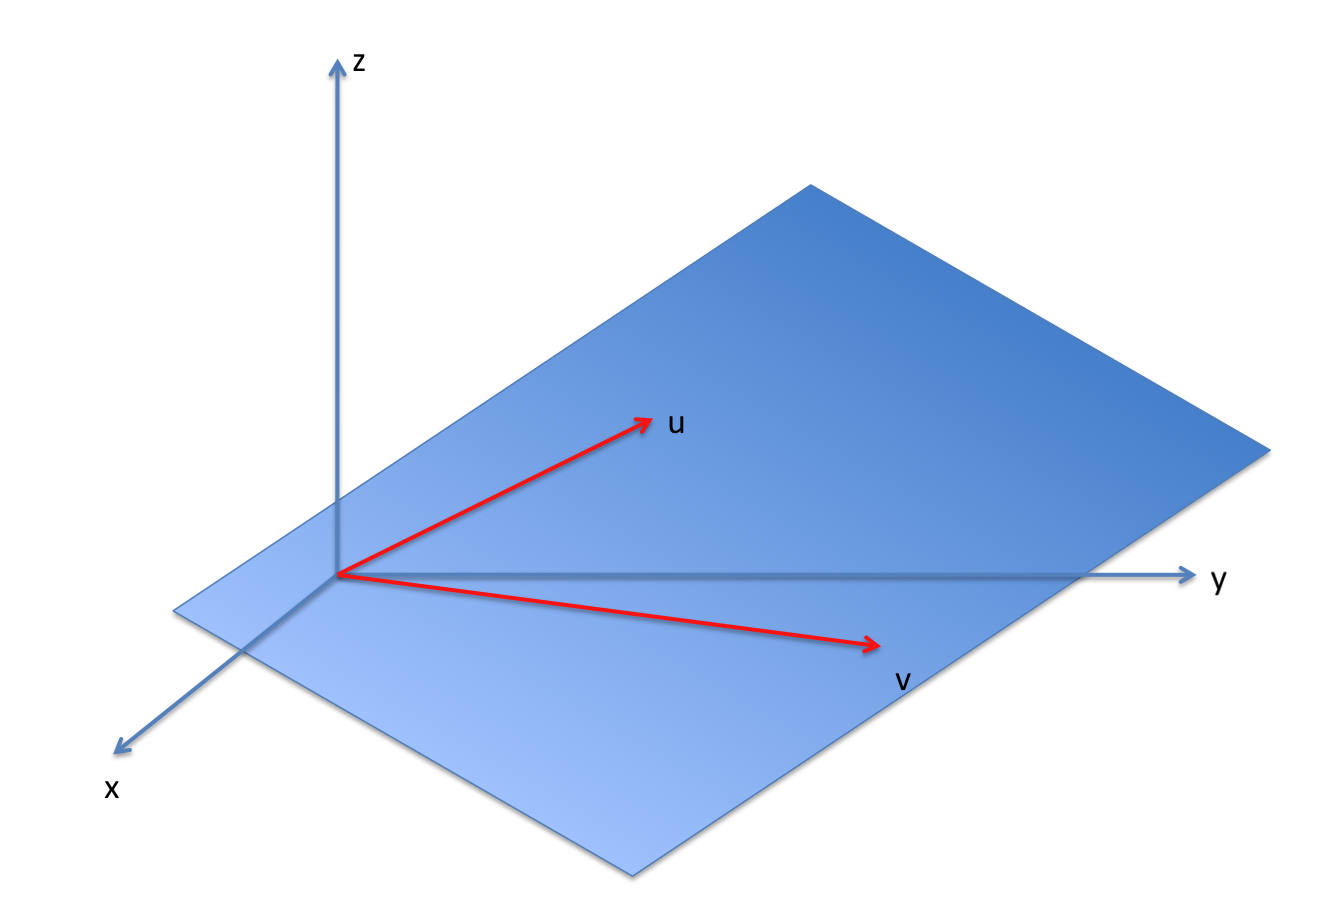
\includegraphics[width=\linewidth]{img/1_3_Plane}
		\end{center}
	\end{multicols}

	Give an example of two distinct, nonzero vectors $\vect{u}$ and $\vect{v}$ in $\R^3$ so that $\Span\{\vect{u},\vect{v}\}$ is \textbf{not} a plane. What is the geometric interpretation of $\Span\{\vect{u},\vect{v}\}$ for your example?
\end{exercise}
\vspace{1.5in}

\clearpage
\begin{exercise} % locations in a qr code as a vector equation

  Quick response (QR) codes are used to display bits in a two
  dimensional array. Each bit is in the shape of a rectangle and is
  either black or white. Smartphone apps take an image of a QR code
  and convert the pixels into a string of characters. There are a
  number of important positions in a QR code including the position
  markers in the lower left, upper left, and upper right of the code.

  The markers help identify the orientation of the code. An example of
  the codes is shown in Figure \ref{fig:qrCodeExample}. In the lower
  left, upper left, and upper right corners are special areas to
  indicate the orientation and location of the box that contains the
  QR code. This is shown in Figure
  \ref{fig:qrCodeExampleDirections}.

  One problem with a QR code is that the image taken by a camera is
  not oriented exactly over the code. The boxes that determine the
  orientation of the code can be used to define vectors that can be
  used to determine the location of a bit in the image of the QR
  code. The vectors that can be calculated represent the vertical
  ($\vec{v}$) and horizontal ($\vec{u}$) directions of the skewed
  image. Given a point in the QR code, it can be expressed as a linear
  combination of the $\vec{v}$ and $\vec{u}$ directions. The
  coefficients for the different directions indicate where the
  locations of certain points are within the QR code.

  \begin{figure}[h]
    %\centering
    \begin{tabular}[h]{p{5cm}@{\hspace{3em}}p{5cm}}
    \qrcode[nolink,level=L,height=5cm]{abcd} &
     \begin{minipage}[h]{5cm}
         \vspace{1.5em}
         
\includegraphics[height=5cm]{img/qrCodeSnapshot}
     \end{minipage}
    \end{tabular}
    \caption{Example of a QR code. The code on the left is the
      original, and the code on the right is the skewed image obtained
      using a mobile phone.}
    \label{fig:qrCodeExample}
  \end{figure}

    \begin{figure}[h]
    \centering
    \begin{tabular}{l@{\hspace{3em}}r}
      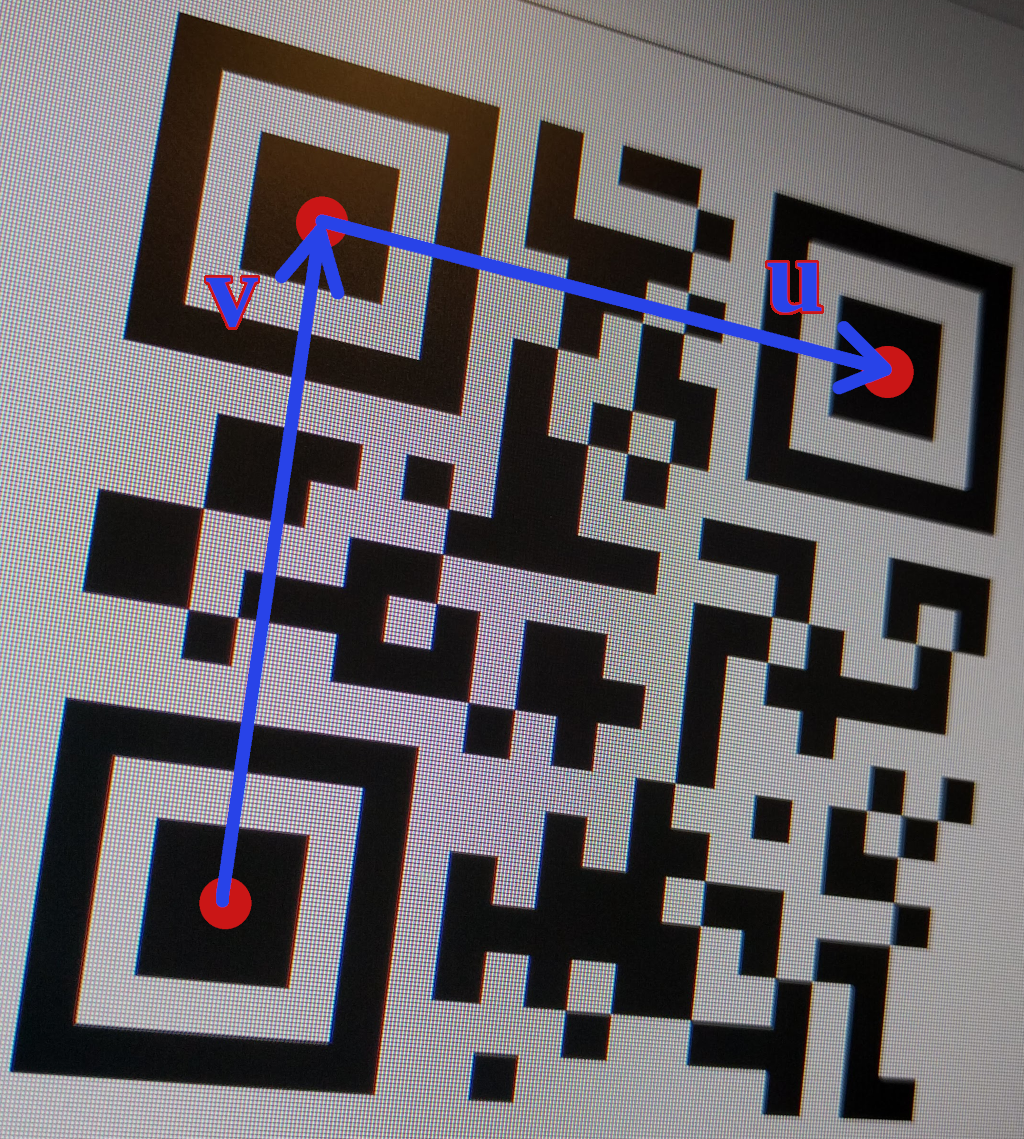
\includegraphics[width=6cm]{img/qrCodeSnapshotUV} &
      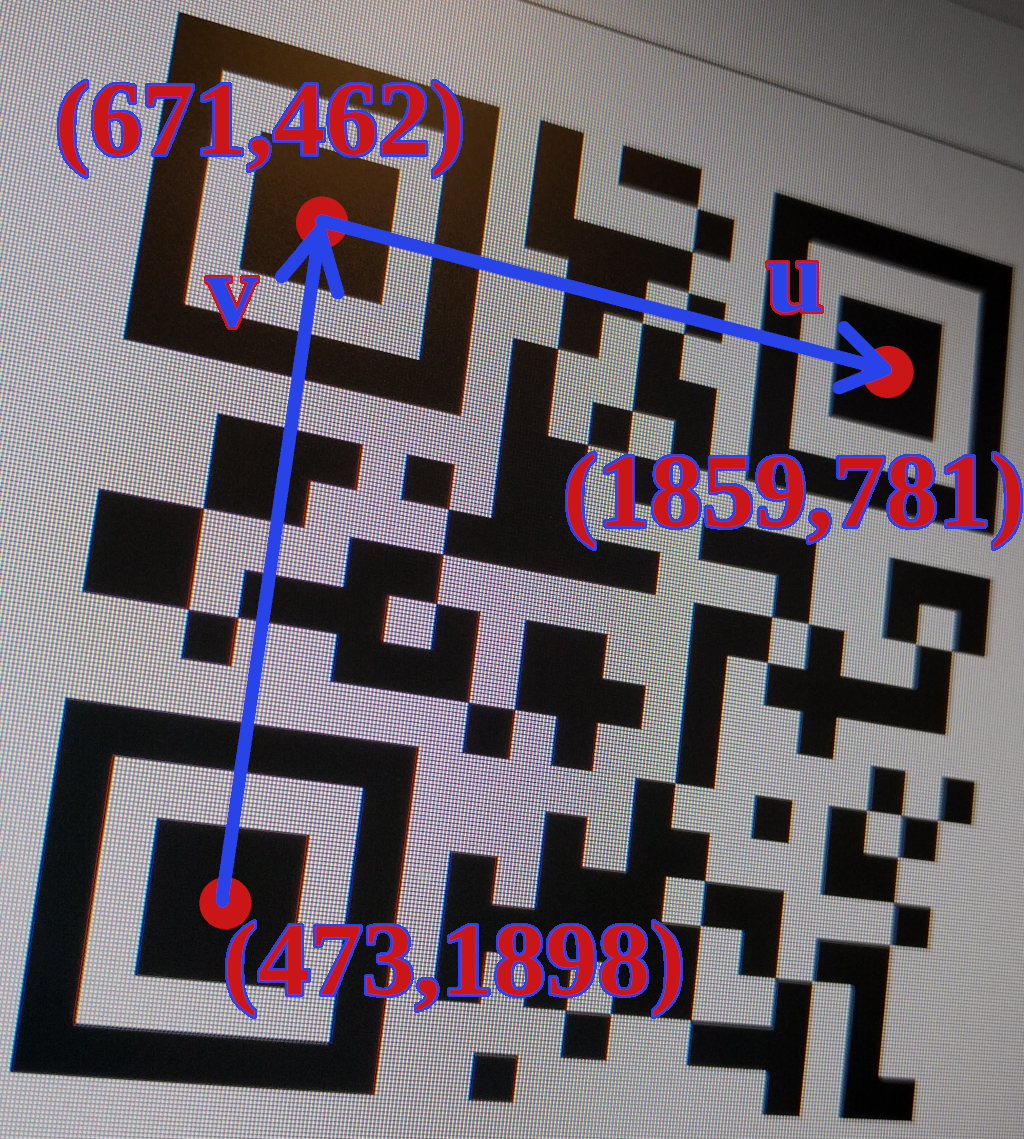
\includegraphics[width=6cm]{img/qrCodeSnapshotUV-coordinates}
    \end{tabular}
    \caption{Example of a QR code. The code on the left indicates the
      horizontal and vertical directions for the image of the
      code. The code on the right indicates the locations of the
      pixels marking the tail and the head of the vectors indicating
      the directions. }
    \label{fig:qrCodeExampleDirections}
  \end{figure}

  \begin{figure}[h]
    \centering
    %\begin{tabular}{l@{\hspace{3em}}r}
      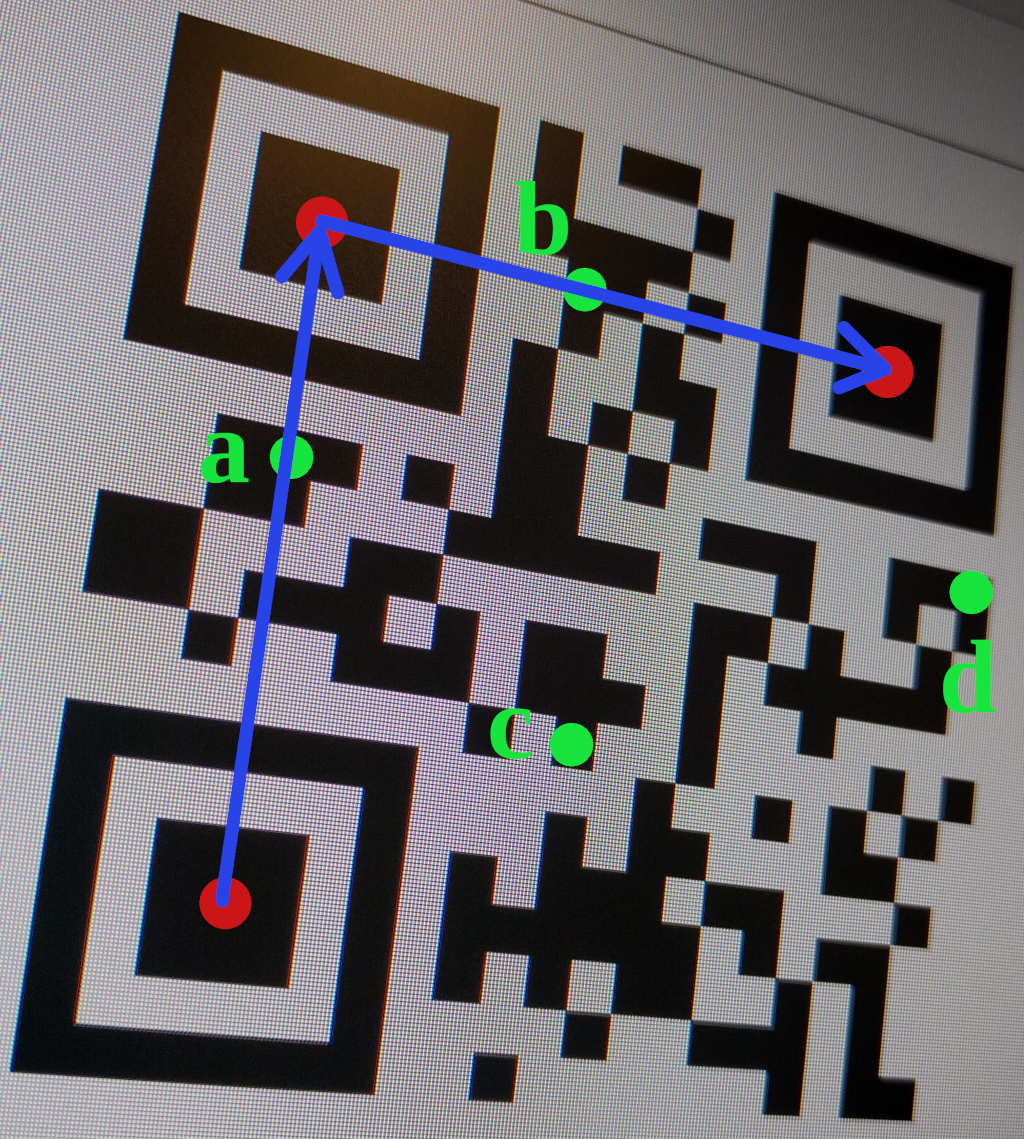
\includegraphics[width=6cm]{img/qrCodeSnapshotUV-points.png}
    %\end{tabular}
    \caption{Example of a QR code. The pixels indicated by points $a$,
    $b$, $c$ and $d$ are locations that provide information about the
    text for the code. Each location should either be a black square
    or a white square.}
    \label{fig:qrCodeExampleLocations}
  \end{figure}

\end{exercise}


\clearpage
\newpage


% SEC 1.4
\section{The Matrix Equation $\boldsymbol{Ax=b}$}
\sectionmark{The Matrix Equation $A\vect{x}=\vect{b}$}
\name[2.25in]

\begin{exercise} % 1.4.3
	A matrix $A$ and column vector $\vect{x}$ are given.
	\begin{align*}
	A &= \begin{bmatrix}6&5\\-3&-4\\7&4\end{bmatrix}, &
	\vect{x} &= \begin{bmatrix}3\\-2\end{bmatrix}
	\end{align*}
	There are two main ways to think about the product $A\vect{x}$.
	\begin{multicols}{2}
		\begin{enumerate}[(a)]
			\item Write the product $A\vect{x}$ as a linear combinations of the columns of $A$ using the entries of $\vect{x}$ as weights. Compute the product.
			\columnbreak
			\item Compute the product $A\vect{x}$ using the row-vector rule. Show your work clearly. \par
			$ A\vect{x} = \begin{bmatrix}6&5\\-3&-4\\7&4\end{bmatrix}\begin{bmatrix}3\\-2\end{bmatrix} = $
		\end{enumerate}
	\end{multicols}
\end{exercise}
\vfill

\begin{boxthm}
	\textbf{Theorem 3.} \\
	If $A$ is an $m\times n$ matrix with columns $\vect{a}_1,\ldots,\vect{a}_n$, and if $\vect{b}$ is in $\R^m$, the matrix equation $A\vect{x}=\vect{b}$ has the same solutions set as the vector equation $x_1\vect{a}_1+x_2\vect{a}_2+\cdots+x_n\vect{a}_n=\vect{b}$ which, in turn, has the same solution set as the system of linear equations whose augmented matrix is $\begin{bmatrix}\vect{a}_1&\vect{a}_2&\cdots&\vect{a}_n&\vect{b}\end{bmatrix}$.
\end{boxthm}

\begin{exercise} % 1.4.11
	Write the augmented matrix that corresponds to the matrix equation $A\vect{x}=\vect{b}$ and solve the system to find $\vect{x}$.
	\begin{align*}
	A &= \begin{bmatrix}1&2&-4\\1&5&2\\2&3&2\end{bmatrix} &
	\vect{b} &= \begin{bmatrix}-17\\22\\13\end{bmatrix}
	\end{align*}
\end{exercise}
\vfill


\newpage


\begin{boxthm}
	\textbf{Theorem 4.} \\
	Let $A$ be an $m\times n$ matrix. Then the following statements are logically equivalent.
	\begin{enumerate}[(a)]\itemsep0em 
		\item For each $\vect{b}$ in $\R^m$, the equation $A\vect{x}=\vect{b}$ has a solution.
		\item Each $\vect{b}$ in $\R^m$ is a linear combination of the columns of $A$.
		\item The columns of $A$ span $\R^m$.
		\item $A$ has a pivot position in every row.
	\end{enumerate}
\end{boxthm}

\begin{exercise} % 1.4.16
	Show that the equation $A\vect{x}=\vect{b}$ does not have a solution for all possible $\vect{b}$, and describe the set of all $b$ for which $A\vect{x}=\vect{b}$ does have a solution.
	\begin{align*}
	A &= \begin{bmatrix}1&-4&-3\\-3&3&0\\4&2&6\end{bmatrix} &
	\vect{b} &= \begin{bmatrix}b_1\\b_2\\b_3\end{bmatrix}
	\end{align*}
	(Hint: Note that by Theorem 4, to show that $A\vect{x}=\vect{b}$ does not have a solution for all $\vect{b}$, you just need to show that $A$ does not have a pivot in every row. However, to determine $\vect{b}$ for which $A\vect{x}=\vect{b}$ does have a solution, you will need to put the augmented matrix $\begin{bmatrix}\vect{a}_1&\vect{a}_2&\vect{a}_3&\vect{b}\end{bmatrix}$ in row echelon form.)
\end{exercise}
\vfill

\begin{exercise} % 1.4.13
	The columns of the matrix $A$ span a plane in $\R^3$. Is $\vect{u}$ in the plane spanned by the columns of $A$? If so, write $\vect{u}$ as a linear combination of the columns of $A$.
	\begin{align*}
	A &= \begin{bmatrix}4&-6\\-3&5\\1&1\end{bmatrix} &
	\vect{u} &= \begin{bmatrix}6\\-3\\9\end{bmatrix}
	\end{align*}
\end{exercise}
\vfill


\newpage

% SEC 1.5
\section{Solution Sets of Linear Systems}
\name[2in]

\begin{boxme}
	The homogeneous equation $A\vect{x}=\vect{0}$ has a nontrivial solution if, and only if, the equation has at least one free variable.
\end{boxme}
\begin{exercise} % 1.5.3
	Determine if the system has a nontrivial solution.
	$$\systeme{-2x_1+6x_2-6x_3=0,-4x_1+8x_2+3x_3=0}$$
\end{exercise}
\vfill

\begin{boxme}
	\begin{multicols}{2}
	To write a solution set in parametric vector form:
	\begin{enumerate}[(1)]\itemsep0em 
		\item Row reduce augmented matrix to RREF
		\item Express basic var. in terms of free var.
		\item Write the solution $\vect{x}$ as a vector whose entries depend on the free variables.
		\item Decompose $\vect{x}$ into a linear combination of vectors using free variables as parameters.
	\end{enumerate}
	
	\columnbreak
	
	\textbf{Example.}
	Solution set: $\begin{cases}x_1=3-2x_3 \\ x_2 = -4 \\ x_3 \text{ is free}\end{cases}$
	$$\vect{x}=\begin{bmatrix}x_1\\x_2\\x_3\end{bmatrix}
	=\begin{bmatrix}3-2x_3\\-4\\x_3\end{bmatrix}
	=\begin{bmatrix}3\\-4\\0\end{bmatrix} +x_3\begin{bmatrix}-2\\0\\1\end{bmatrix}$$
	\end{multicols}
\end{boxme}
\begin{exercise} % 1.5.7
	The matrix $A$ is given below along with its reduced echelon form and the associated system of equations of the matrix equation $A\vect{x}=\vect{0}$.
	$$A=\begin{bmatrix}1&4&-3&5\\1&5&-5&7\end{bmatrix}\xrightarrow{\text{RREF}}
	\begin{bmatrix}1&0&5&-3\\0&1&-2&2\end{bmatrix}\xrightarrow{\text{System}}
	\systeme{x_1 + 5x_3 - 3x_4 = 0, x_2 - 2x_3 + 2x_4 = 0} $$
	\begin{enumerate}[(a)]
		\item Describe the solution set of $\Axz$ in parametric vector form.
		\vfill
		\item Circle the best answer. \par
		The solution set of $A\vect{x}=\vect{0}$ is a: \quad \textbf{Single Vector} \qquad \textbf{Line} \qquad \textbf{Plane} \qquad \textbf{None of these}
	\end{enumerate}
\end{exercise}


\newpage


\begin{exercise} % 1.5.15
	\textbf{Compare $\Axb$ and $\Axz$} \par
	The solution sets of the systems of linear equations below are given.
	
	\noindent	
	\begin{tabular}{c|c}
		\parbox{0.5\linewidth}{%
			\begin{align*}
			\systeme{2x_1+2x_2+4x_3=8,-4x_1-4x_2-8x_3=-16,-3x_2+6x_3=9}&&
			\begin{cases}x_1 = 7-4x_3 \\ x_2 =-3+2x_3 \\ x_3 \text{ is free}\end{cases}
			\end{align*}}
		&
		\parbox{0.5\linewidth}{%
			\begin{align*}
			\systeme{2x_1+2x_2+4x_3=0,-4x_1-4x_2-8x_3=0,-3x_2+6x_3=0}&&
			\begin{cases}x_1 = -4x_3 \\ x_2 =2x_3 \\ x_3 \text{ is free}\end{cases}
			\end{align*}}
	\end{tabular}
	
	\begin{enumerate}[(a)]
		\item Write the solution sets in parametric vector form.
		\begin{multicols}{2}
			\begin{enumerate}[(i)]
				\item First System
				\item Second System
			\end{enumerate}
		\end{multicols}
		\vfill
		\item Provide a geometric comparison between the solution sets of the two systems. (Are the solution sets single vectors? Lines? Planes? Something else? How are they related to one another?)
		\vspace{1in}
	\end{enumerate}
\end{exercise}

\begin{exercise} % 1.5.
	A $3\times 4$ matrix $A$ has 3 pivot positions.
%	e.g.
%	$\begin{bmatrix}
%	\blacksquare	& *	& 0				& *				& * \\ 
%	0				& 0	& \blacksquare	& * 			& * \\ 
%	0				& 0	& 0				& \blacksquare	& *
%	\end{bmatrix}$
	\begin{multicols}{2}
		\begin{enumerate}[(a)]
			\item Does the equation $\Axz$ have a nontrivial solution? How do you know?
			\item Does the equation $\Axb$ have at least one solution for any choice of $\vect{b}$ in $\R^3$? How do you know?
		\end{enumerate}
	\end{multicols}
\end{exercise}
\vfill


\newpage


% SEC 1.6
\section{Applications of Linear Systems}
\names[4]


\begin{exercise} % 1.6.3 textbook
	Consider an economy with 3 sectors, Chemicals \& Metals, Fuels \& Power, and Machinery. Chemicals sells 30\% of its output to Fuels and 50\% to Machinery and retains the rest. Fuels sells 80\% of its output to Chemicals and 10\% to Machinery and retains the rest. Machinery sells 40\% to Chemicals and 40\% to Fuels and retains the rest.
	\begin{enumerate}[(a)]
		\item Construct the exchange table for this economy. \par
			\renewcommand{\arraystretch}{2}
			\begin{tabular}{|c|c|c|c|}
				\hline
				\textbf{Chem}	& \textbf{Fuels}	& \textbf{Mach}	& \textbf{Purchased by:} \\ \hline
				&	&	& Chem \\ \hline
				&	&	& Fuel \\ \hline
				&	&	& Mach \\ \hline
			\end{tabular}
		\item Develop a system of equations that leads to prices at which each sector's income matches its expenses using $p_C$, $p_F$, and $p_M$ for the price of Chemicals, Fuels, and Machinery outputs, respectively. Then write the augmented matrix that can be row reduced to find these prices.
		\vfill
		\item Find a set of equilibrium prices when the price for the Machinery ouput is 100 units.
		\vfill
	\end{enumerate}
\end{exercise}


\newpage


\begin{exercise} % 1.6.7
	Alka-Seltzer contains sodium bicarbonate (\ce{NaHCO3}) and citric acid (\ce{H3C6H5O7}). When a tablet is dissolved in water, the following reaction produces sodium citrate, water, and carbon dioxide (gas):
	\begin{center}
		\ce{NaHCO3 + H3C6H5O7 -> Na3C6H5O7 + H2O + CO2} \\
		%\ce{3NaHCO3 + 1H3C6H5O7 -> 1Na3C6H5O7 + 3H2O + 3CO2}
	\end{center}
	Balance the chemical equation. (Hint: there are 5 unknowns---one for each of the 5 molecules. The column vectors you construct will each contain 4 entries---one for each type of atom present, Na, H, C, and O)
\end{exercise}
\vfill

%\begin{exercise} % 1.6.9
%	Balance the chemical equation. Assume the coefficient of NO is 90.
%	\begin{center}
%		\ce{PbN6 + CrMn2O8 -> Pb3O4 + Cr2O3 + MnO2 + NO}
%		%\ce{15PbN6 + 44CrMn2O8 -> 5Pb3O4 + 22Cr2O3 + 88MnO2 + 90NO}
%	\end{center}
%\end{exercise}
%\vfill


\begin{exercise} % 1.6.11
	\begin{enumerate}[(a)]
		\item Find the general flow pattern of the network shown in the figure. \par
		% ADD IN TABLE FOR FLOW IN & OUT OF EACH NODE
			\hfill
			\begin{tikzpicture}[shorten >=1pt,node distance=2cm,on grid,auto]
			\tikzset{->-/.style={decoration={markings,mark=at position .6 with {\arrow{stealth}}},postaction={decorate}}}
			\tikzstyle{every edge}=[draw,->-,line width=1pt]
			\tikzset{junction/.style={fill=black,draw=none,inner sep=0pt, minimum size=5pt,circle}}
			% Place Nodes
			\node (OUT1) {70};
			\node[junction] (A) [right=of OUT1] {};
			\node[junction] (B) [below right=of A] {};
			\node[junction] (C) [below left=of B] {};
			\node (IN) [left=of C] {90};
			\node (OUT2) [right=of B] {$x_4$};
			% Label nodes
			\draw (A) node[above right] {A};
			\draw (B) node[above right] {B};
			\draw (C) node[below right] {C};
			% Draw flow paths
			\path
			(A) edge (OUT1)
			(B) edge node[above right] {$x_3$} (A)
			(B) edge (OUT2)
			(C) edge node[below right] {$x_2$} (B)
			(C) edge node {$x_1$} (A)
			(IN) edge (C);
			\end{tikzpicture}
		\vfill
		\item Assuming that the flows are all nonnegative, what is the largest possible value for $x_3$?
		\vspace{2em}
	\end{enumerate}
% Solution
%$\begin{cases}
%	x_1 = 70 - x_3 \\
%	x_2 = 20 + x_3 \\
%	x_3 \text{ is free} \\
%	x_4 = 20
%	\end{cases}$
\end{exercise}


\newpage


% SEC 1.7
\section{Linear Independence}
\name

\begin{boxdef}
	An indexed set of vectors $\{\vect{v}_1,\ldots,\vect{v}_p\}$ in $\R^n$ is said to be \textbf{linearly independent} if the vector equation
	$$ x_1\vect{v}_1 + x_2\vect{v}_2 + \cdots + x_p\vect{v}_p = \vect{0} $$
	has only the trivial solution. The set $\{\vect{v}_1,\ldots,\vect{v}_p\}$ is said to be \textbf{linearly dependent} if there exist weights $c_1,\ldots,c_p$ not all zero, such that
	\begin{align*}
	c_1\vect{v}_1 + c_2\vect{v}_2 + \cdots + c_p\vect{v}_p = \vect{0}. \tag{\dag}
	\end{align*}
	The equation $(\dag)$ is called a \textbf{linear dependence relation}. (Note that each linear dependence relation corresponds to a nontrivial solution of the vector equation.)
\end{boxdef}

\begin{exercise} % 1.7.
	Determine by inspection if the given vectors are linearly independent. If they are not, write a linear dependence relation to prove they are linearly dependent.
	\begin{multicols}{2}
		\begin{enumerate}[(a)]
			\item $$\vect{u}=\begin{bmatrix}3\\-2\end{bmatrix}, \vect{v}=\begin{bmatrix}-9\\6\end{bmatrix}$$
			\item $$\vect{w}=\begin{bmatrix}0\\0\\0\\0\end{bmatrix}, \vect{z}=\begin{bmatrix}3\\3\\3\\3\end{bmatrix}$$
		\end{enumerate}
	\end{multicols}
\end{exercise}
\vfill


\begin{boxdef}
	The columns of a matrix $A$ are linearly independent if, and only if, the equation $\Axz$ has \emph{only} the trivial solution.
\end{boxdef}
\begin{exercise} % 1.7.5
	A matrix is given along with its reduced echelon form. Determine if the columns of the matrix are linearly independent. Explain your answer.
	\begin{multicols}{2}
		\begin{enumerate}[(a)]
			\item
				\begin{align*}
				A = \begin{bmatrix}0&-3&9\\2&1&-7\\-1&4&-4\\1&-4&-2\end{bmatrix}
				&\xrightarrow{\text{RREF}}
				\begin{bmatrix}1&0&0\\0&1&0\\0&0&1\\0&0&0\end{bmatrix}
				\end{align*}
			\item 
				\begin{align*}
				B = \begin{bmatrix}1&-3&5&0\\3&-9&6&1\\2&-6&0&1\end{bmatrix}
				&\xrightarrow{\text{RREF}}
				\begin{bmatrix}1&-3&0&0\\0&0&1&0\\0&0&0&1\end{bmatrix}
				\end{align*}
		\end{enumerate}
	\end{multicols}
\end{exercise}
\vfill


\newpage


\begin{exercise} % 1.7.31
	Given $A=\begin{bmatrix}2&4&6\\-6&1&-5\\-4&-2&-6\\4&0&4\end{bmatrix}$, observe that the 3rd column is the sum of the 1st and 2nd columns.
		\begin{enumerate}[(a)]
			\item Without performing row operations, give a nontrivial solution of $\Axz$.
			\vfill
			\item Write $A\vect{x}$ as a linear combination of the columns of $A$ using the entries of your solution to part (a) as weights. Simplify the expression to show that your solution to part (a) is correct.
			\vfill
		\end{enumerate}
\end{exercise}


\begin{boxthm}
	\textbf{Theorem 7.}
	\textbf{Characterization of Linearly Independent Sets (Short Version)} \\
	An indexed set $S=\{\vect{v}_1,\ldots,\vect{v}_p\}$ of two or more vectors is linearly dependent if, and only if, at least one of the vectors in $S$ is a linear combination of the others.
\end{boxthm}
\begin{boxthm}
	\textbf{Theorem 8.} \\
	If a set contains more vectors than there are entries in each vector, then the set is linearly dependent. That is, any set $\{\vect{v}_1,\ldots,\vect{v}_p\}$ in $\R^n$ is linearly dependent if $p>n$.
\end{boxthm}
\begin{exercise} % 1.7.Custom
	Determine if the following vectors are linearly independent or linearly dependent. Explain your answer. Be sure to reference the appropriate theorem.
		\begin{multicols}{2}
			\begin{enumerate}[(a)]
				\item
					$$
					\begin{bmatrix} 2\\1\\-5 \end{bmatrix},
					\begin{bmatrix} 5\\-7\\3 \end{bmatrix},
					\begin{bmatrix} -6\\-3\\15 \end{bmatrix}
					$$
					Circle one and explain your answer:
					\begin{center}
						\shortstack{\textbf{Linearly}\\ \textbf{Independent}} \qquad
						\shortstack{\textbf{Linearly}\\ \textbf{Dependent}}
					\end{center}
				
				\columnbreak
				
				\item
					$$
					\begin{bmatrix}  2\\ 3\\ 5\\ 7 \end{bmatrix},
					\begin{bmatrix} 11\\13\\17\\19 \end{bmatrix},
					\begin{bmatrix} 23\\29\\31\\37 \end{bmatrix},
					\begin{bmatrix} 41\\43\\47\\53 \end{bmatrix},
					\begin{bmatrix} 59\\61\\67\\71 \end{bmatrix}
					$$
					Circle one and explain your answer:
					\begin{center}
						\shortstack{\textbf{Linearly}\\ \textbf{Independent}} \qquad
						\shortstack{\textbf{Linearly}\\ \textbf{Dependent}}
					\end{center}
			\end{enumerate}
		\end{multicols}
\end{exercise}
\vfill


%\begin{exercise} % 1.7.Custom
%	If you have a linearly independent set of vectors, $\{\vect{u},\vect{v}\}$ and you know that $\vect{w}$ is in $\Span\{\vect{u},\vect{v}\}$, can you determine whether the set $\{\vect{u},\vect{v},\vect{w}\}$ is linearly independent or not?
%\end{exercise}
%\vfill


\newpage


% SEC 1.8
\section[Introduction to Linear Transformations]{Intro to Linear Transformations}
\name[2in]

\begin{boxdef}
	A \textbf{transformation} $T:\R^n\to\R^m$ is a rule that assigns to each vector in $\R^n$ a vector $T(\vect{x})$ in $\R^m$. The set $\R^n$ is called the \textbf{domain} of $T$, and $\R^m$ is called the \textbf{codomain} of $T$. For $\vect{x}\in\R^n$, the vector $T(\vect{x})$ is called the \textbf{image} of $\vect{x}$ (under the action of $T$). The set of all images $T(\vect{x})$ is called the \textbf{range} of $T$.
\end{boxdef}

\begin{exercise} % 1.8.Custom
	Suppose we define a transformation $T$ by $T(\vect{x})=\Ax$ where $A=\begin{bmatrix}1&3&1\\2&6&8\\0&0&0\\0&0&1\end{bmatrix}$.
	\begin{enumerate}[(a)]
		\item What is the domain of $T$?
		\vspace{1em}
		\item What is the codomain of $T$?
		\vspace{1em}
		\item Are the range and codomain of $T$ the same? Why or why not? \par
		Hint: think of the range as all possible linear combinations of the columns of $A$.
	\end{enumerate}
\end{exercise}
\vfill



\begin{exercise} % 1.8.9
	Find all $\vect{x}$ in $\R^4$ that are mapped into the zero vector by the transformation $\vect{x}\mapsto\Ax$ for the given matrix $A$.
	$$ \begin{bmatrix} 1&-5&18&-3 \\ 0&1&-5&2 \\ 4&-16&52&-4 \end{bmatrix}$$
	% Solution
	%$$ x_3\begin{bmatrix}7\\5\\1\\0\end{bmatrix} + x_4\begin{bmatrix}-7\\-2\\0\\1\end{bmatrix}$$
\end{exercise}
\vfill


\newpage


\begin{boxme}
	A transformation $T$ is \textbf{linear} if:
	\begin{enumerate}[(i)]\itemsep=0pt
		\item $T(\vect{u}+\vect{v}) = T(\vect{u})+T(\vect{v})$ for all $\vect{u},\vect{v}$ in the domain of $T$.
		\item $T(c\vect{u}) = cT(\vect{u})$ for all scalars $c$ and all $\vect{u}$ in the domain of $T$.
	\end{enumerate}
	This implies the following:
	\begin{enumerate}[(i)]\itemsep=0pt
		\item $T(\vect{0})=\vect{0}.$
		\item $T(c\vect{u}+d\vect{v}) = cT(\vect{u})+dT(\vect{v})$ for all scalars $c,d$ and all vectors  $\vect{u},\vect{v}$ in the domain of $T$.
	\end{enumerate}
	Note: to prove a transformation $T$ is linear, you only need to show $T(c\vect{u}+d\vect{v}) = cT(\vect{u})+dT(\vect{v})$.
\end{boxme}

\begin{exercise} % 1.8.17
	A linear transformation $T:\R^2\to\R^2$ maps the vector $\vect{u}=\begin{bmatrix}6\\3\end{bmatrix}$ to $\begin{bmatrix}5\\1\end{bmatrix}$ and maps the vector $\vect{v}=\begin{bmatrix}3\\3\end{bmatrix}$ to $\begin{bmatrix}-1\\3\end{bmatrix}$. Use that fact that $T$ is linear to find the image of $3\vect{u}+4\vect{v}$ under $T$.
\end{exercise}
\vfill


\begin{exercise} % 1.8.15
	The vectors $\vect{u}=\begin{bmatrix}-2\\5\end{bmatrix}$ and $\vect{v}=\begin{bmatrix}3\\-1\end{bmatrix}$ are plotted on the graph below.
	\begin{enumerate}[(a)]
		\item Plot $T(\vect{u})$ and $T(\vect{v})$ under the given transformation $T$.
		
		$$ \Tx = \begin{bmatrix}1&0\\0&0\end{bmatrix}\begin{bmatrix}x_1\\x_2\end{bmatrix} $$
		
		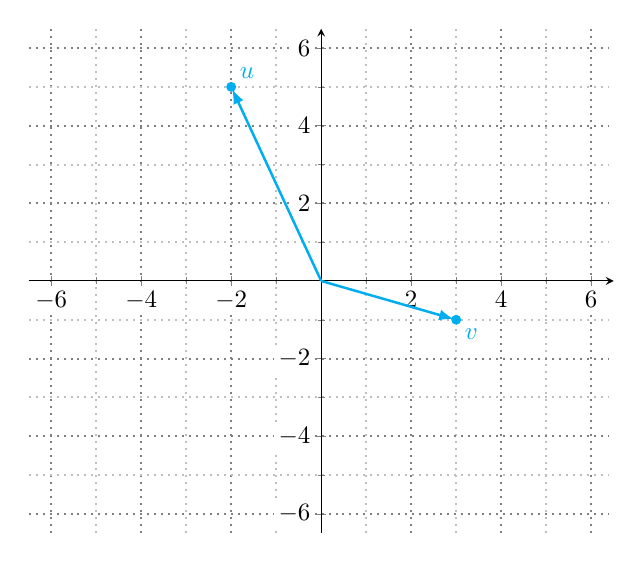
\begin{tikzpicture}[scale=.9]
		% Set u and v
		\pgfmathtruncatemacro{\ux}{-2}
		\pgfmathtruncatemacro{\uy}{5}
		\pgfmathtruncatemacro{\vx}{3}
		\pgfmathtruncatemacro{\vy}{-1}
		% Begin Axis
		\begin{axis}[axis x line=center, axis y line=middle,
		xmin=-6.5, xmax=6.5,
		ymin=-6.5, ymax=6.5,
		xtick={-6,-4,...,6}, ytick={-6,-4,...,6},
		ticklabel style={draw=none, inner sep=2pt, fill=white, text opacity=1},
		scale only axis, width=3.25in,
		grid=both, minor tick num=1,
		major grid style={line width=.8pt, draw=gray, dotted},
		minor grid style={line width=.8pt, draw=gray!50, dotted}]
		% Draw vectors
		\draw[-latex, shorten >=.25ex, line width=1pt, cyan] (0,0) -- (\ux,\uy);
		\fill[cyan] (\ux,\uy) circle (2pt) node[above right, fill=white, rounded corners=0.2cm] {$\vect{u}$};
		\draw[-latex, shorten >=.25ex, line width=1pt, cyan] (0,0) -- (\vx,\vy);
		\fill[cyan] (\vx,\vy) circle (2pt) node[below right, fill=white, rounded corners=0.2cm] {$\vect{v}$};
		\end{axis}
		\end{tikzpicture}
		
		\item Describe geometrically what $T$ does to each vector $\vect{x}$ in $\R^2$. (Is it a rotation? Reflection? Projection? Shear? Dilation? Contraction? Something else?)
	\end{enumerate}
\end{exercise}
\vspace{2em}


\newpage


% SEC 1.9
\section[The Matrix of a Linear Transformation]{Matrix of a Linear Transformation}
\name[2in]

\begin{boxthm}
	\textbf{Theorem 10.} \\
	Let $T:\R^n\to\R^m$ be a linear transformation. Then there exists a unique matrix $A$ such that $\Tx=\Ax$ for all $\vect{x}$ in $\R^n$. In fact, $A$ is the $m\times n$ matrix whose $j$th column is the vector $\Te{j}$, where $\ve{j}$ is the $j$th column of the identity matrix in $\R^n$:
	$$ A = \begin{bmatrix}\Te1 & \cdots & \Te{n}\end{bmatrix}. $$
\end{boxthm}

\begin{exercise} % 1.9.2
	Suppose $\Tmap{3}{2}$ is a linear transformation such that $\Te1=(1,3)$, $\Te2=(-5,3)$, and $\Te3=(3,-8)$, where $\ve1$, $\ve2$, and $\ve3$ are the columns of the $3\times 3$ identity matrix, $I_3=\begin{bmatrix}1&0&0\\0&1&0\\0&0&1\end{bmatrix}$. Find the standard matrix of $T$.
\end{exercise}
\vfill


\begin{exercise} % 1.9.13
	Let $\Tmap{2}{2}$ be a linear transformation such that $\Te1$ and $\Te2$ are the vectors shown in the figure.
	
	\begin{multicols}{2}
		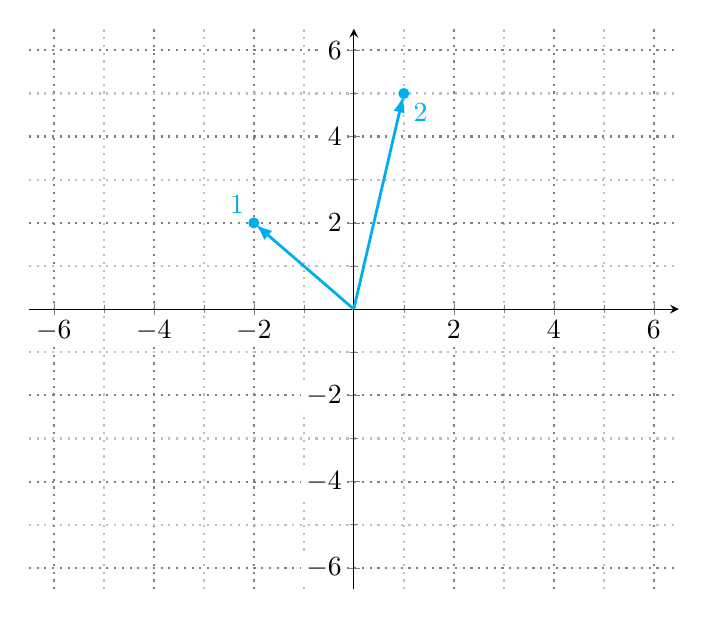
\begin{tikzpicture}[scale=1]
		% Set u and v
		\pgfmathtruncatemacro{\ux}{-2}
		\pgfmathtruncatemacro{\uy}{2}
		\pgfmathtruncatemacro{\vx}{1}
		\pgfmathtruncatemacro{\vy}{5}
		% Begin Axis
		\begin{axis}[axis x line=center, axis y line=middle,
		xmin=-6.5, xmax=6.5,
		ymin=-6.5, ymax=6.5,
		xtick={-6,-4,...,6}, ytick={-6,-4,...,6},
		ticklabel style={draw=none, inner sep=2pt, fill=white, text opacity=1},
		scale only axis, width=3.25in,
		grid=both, minor tick num=1,
		major grid style={line width=.8pt, draw=gray, dotted},
		minor grid style={line width=.8pt, draw=gray!50, dotted}]
		% Draw vectors
		\draw[-latex, shorten >=.25ex, line width=1pt, cyan] (0,0) -- (\ux,\uy);
		\fill[cyan] (\ux,\uy) circle (2pt) node[above left, fill=white, rounded corners=0.2cm] {$\Te1$};
		\draw[-latex, shorten >=.25ex, line width=1pt, cyan] (0,0) -- (\vx,\vy);
		\fill[cyan] (\vx,\vy) circle (2pt) node[below right, fill=white, rounded corners=0.2cm] {$\Te2$};
		\end{axis}
		\end{tikzpicture}
		
		\columnbreak
		
		\begin{enumerate}[(a)]
			\item Using the figure, sketch the vector $T(-2,1)$.
			\vspace{1in}
			\item Write the standard matrix for the linear transformation.
			
				\begin{align*}
				A &=	\huge\begin{bmatrix}
						\phantom{-2}	& \phantom{2} \\
						\phantom{1}		& \phantom{5} \\
						\end{bmatrix}
				\end{align*}
		\end{enumerate}
	\end{multicols}
\end{exercise}


\newpage


\begin{boxdef}
	A mapping $\Tmap{n}{m}$ is said to be \textbf{onto} $\R^m$ if each $\vect{b}$ in $\R^m$ is the image of \emph{at least one} $\vect{x}$ in $\R^n$. The mapping is said to be \textbf{one-to-one} if each $\vect{b}$ in $\R^m$ is the image of \emph{at most one} $\vect{x}$ in $\R^n$.
\end{boxdef}

\begin{boxthm}
	\textbf{Theorem 12.} \\
	Let $T:\R^n\to\R^m$ be a linear transformation, and let $A$ be the standard matrix for $T$. Then:
	\begin{enumerate}[(a)]
		\item $T$ maps $\R^n$ onto $\R^m$ if, and only if, the columns of $A$ span $\R^m$;
		\item $T$ is one-to-one if, and only if, the columns of $A$ are linearly independent.
	\end{enumerate}
\end{boxthm}

\begin{exercise} % 1.9.Custom
	A linear transformation $\Tmap{4}{3}$ has standard matrix $A$. The reduced row echelon form of $A$ is given below.
	$$\begin{bmatrix}1&0&-5&0\\0&1&2&0\\0&0&0&1\end{bmatrix}$$
	\begin{multicols}{2}
		\begin{enumerate}[(a)]
			\item Is $T$ one-to-one? Explain.
			\item Does $T$ map $\R^4$ onto $\R^3$? Explain.
		\end{enumerate}
	\end{multicols}
\end{exercise}
\vfill


\begin{exercise} % 1.9.7
	The standard matrix for rotation about the origin by an angle $\theta$ is $A=\RotMat$. This is because the transformation affects $\ve1$ and $\ve2$ in the following way:
	\begin{align*}
	\begin{bmatrix}1\\0\end{bmatrix} &\mapsto
	\begin{bmatrix} \cos\theta\\ \sin\theta \end{bmatrix} &
	\begin{bmatrix}0\\1\end{bmatrix} &\mapsto
	\begin{bmatrix} -\sin\theta\\ \cos\theta \end{bmatrix}.
	\end{align*}
	Find the standard matrix for the transformation that rotates points by $\frac{\pi}{3}$ radians and then reflects them over the horizontal $x_1$-axis. Simplify any trigonometric expressions.
\end{exercise}
\vfill


\newpage
